% ── Section 5: Oxygen case-study results ─────────────────────────────
\section{Oxygen Case Study: A Compact Transfer Benchmark}
\label{sec:oxygen}

Dissolved oxygen provides a second test of the reconstruction workflow developed for
chlorophyll. It is also locally relevant in its own right: oxygen variability in Tongoy Bay is
connected to the environmental conditions affecting scallop aquaculture
\citep{ramajo2019scallops}, and low-oxygen alerts are already used operationally by local
aquaculture actors \citep{ceaza_tongoy_oxygen_alerts_2024}. The purpose of this section is
therefore twofold: to evaluate whether the same benchmark ladder transfers to another sensor, and,
if it does, to identify what changes in the results.

The oxygen benchmark is deliberately more compact than the
chlorophyll case study. We evaluate the same model ladder, but the main claims
are restricted to an artificial-gap range $L=1$--30. This support contains
406 artificial gaps and 2912 hidden target days.

\subsection{Artificial-gap benchmark}
\label{sec:oxygen_benchmark}

Figure~\ref{fig:oxygen_benchmark_primary} summarizes the oxygen benchmark. Linear
interpolation is again the relevant floor: it clearly improves on monthly climatology and
persistence, with a pooled MAE of 0.733~mg/L. The best external-only
tabular configuration has MAE 0.847~mg/L, about 15.5\% worse than interpolation. Thus, as in the
chlorophyll case, external gridded physical predictors alone do not provide a reliable replacement
for local target continuity inside the bay.

The Gaussian process has a MAE of 0.738~mg/L and its
paired confidence interval includes zero, so it is best read as a statistical tie with
interpolation. The gap-edge residual model reaches near-parity at some medium and longer
gap lengths, but it does not provide an overall improvement over interpolation on the considered
range.

The only method that clearly improves on interpolation in the pooled oxygen benchmark is TS-ICL.
The target-only TS-ICL model is better than interpolation at the point-estimate level, but its
paired improvement is not fully resolved. The strongest audited version uses physical covariate
channels, including SST, wind, solar radiation and
current. This version reaches MAE 0.675~mg/L, an 8.0\% reduction relative to
interpolation, with a 95\% gap-cluster bootstrap confidence interval of 4.5--11.4\%.

The broad chlorophyll conclusion therefore transfers only in part: interpolation remains a strong
baseline, external tabular predictors alone do not clear it in the pooled benchmark, and the
zero-shot foundation model gives the strongest pooled reconstruction result. The failure mode,
however, is different and is analysed in Section~\ref{sec:oxygen_tails}. One visible exception in
Figure~\ref{fig:oxygen_benchmark_primary}A is the external-tabular performance at $L=30$; this
stratum contains only 15 gaps, and a robustness audit showed that the apparent reversal is driven
by a small number of high-error interpolation cases, it is therefore treated as diagnostic.

\begin{figure}[h]
  \centering
  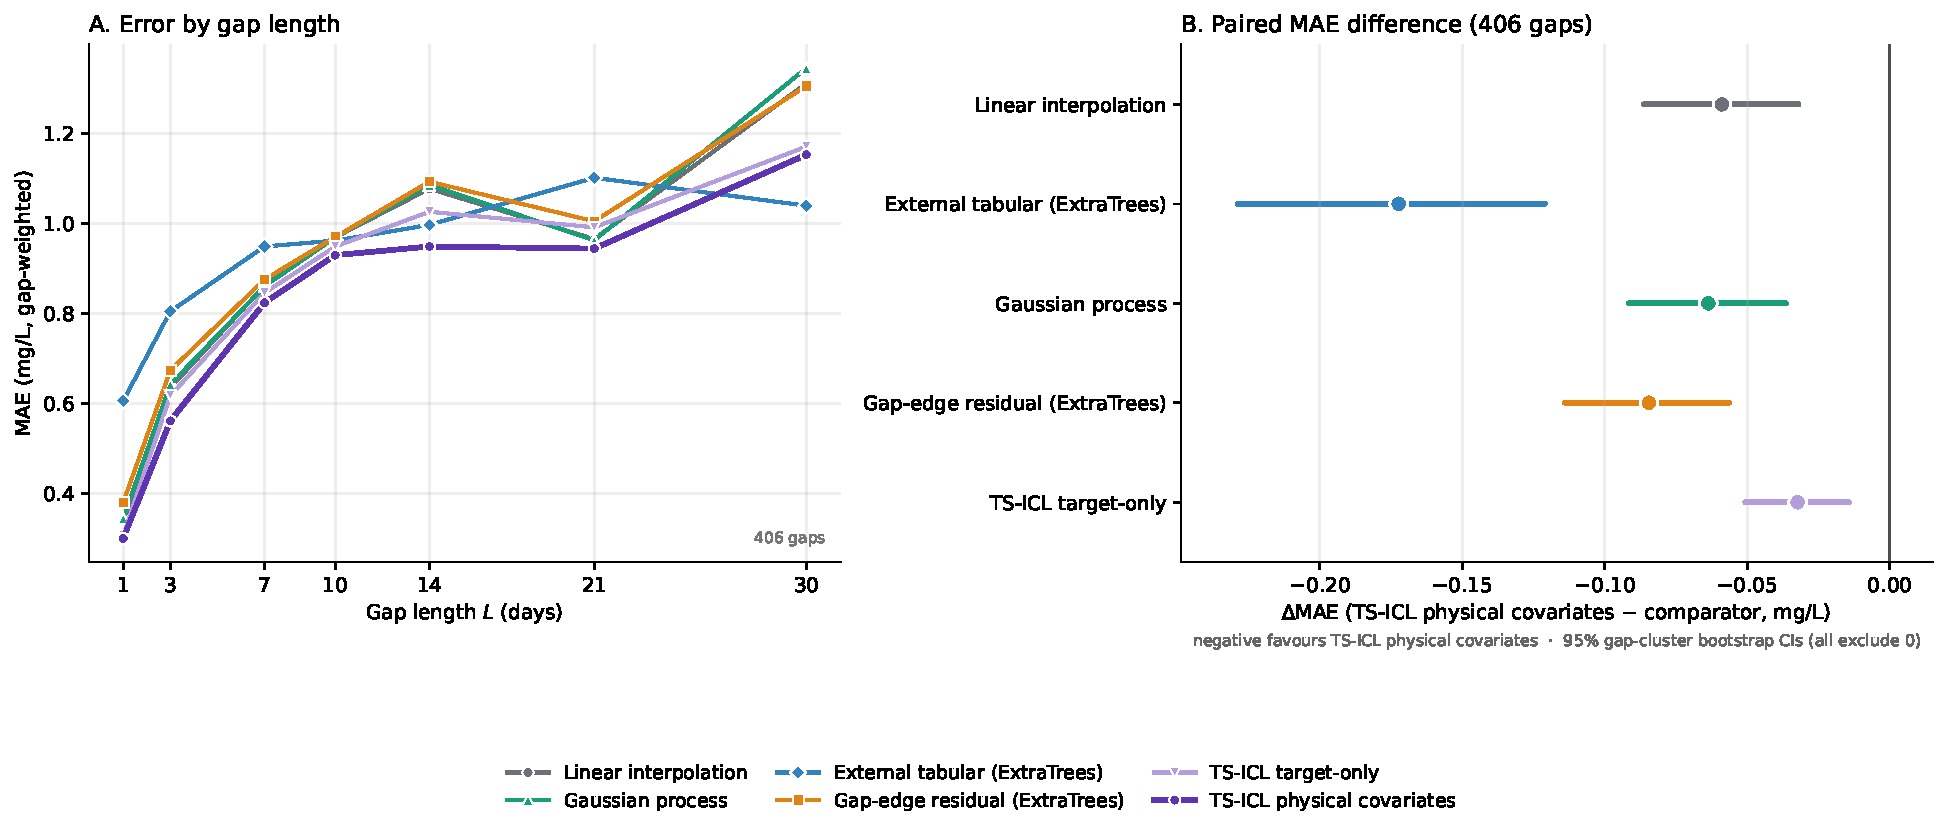
\includegraphics[width=\textwidth]{figures/fig_oxygen_benchmark_primary_v3.pdf}
  \caption{Dissolved-oxygen artificial-gap benchmark.
  (A) Mean absolute error in mg/L by gap length. (B) Pooled paired MAE
  differences between TS-ICL physical covariates and each comparator.}
  \label{fig:oxygen_benchmark_primary}
\end{figure}

\subsection{Physical covariates and distribution-tail limitations}
\label{sec:oxygen_tails}

Running TS-ICL with different covariate arms probes which physical information channels are useful
for oxygen reconstruction. The most informative result concerns current and transport variables:
when added to the broader physical covariate bundle, they do not produce a resolved improvement,
but in isolation the current-only arm is the strongest single-family TS-ICL arm. The
interpretation is that current-derived information is useful, but largely redundant with what the
combined SST, wind and radiation bundle already captures.

TS-ICL's pooled improvement over interpolation is not uniform across the oxygen distribution
(Figure~\ref{fig:oxygen_tail_diagnostics}). The gain is concentrated in the middle of the empirical
oxygen distribution, especially the p10--p25 and p25--p50 bands. At the point-estimate level,
TS-ICL is worse than interpolation in both tails. 

The persistence split sharpens the same point. The largest diagnostic failures occur in sustained
tail runs rather than isolated tail excursions, especially in the sustained high tail. That stratum
is small, so the magnitude should be interpreted cautiously, but the qualitative pattern is
consistent with regression toward the centre of the training distribution: TS-ICL tends to
overpredict low oxygen and underpredict high oxygen.

Two physical associations help interpret the tail pattern but remain exploratory. Same-day solar
radiation is negatively correlated with oxygen ($r=-0.41$), so a simple productivity-driven
high-oxygen explanation is not supported. The low-oxygen tail is enriched in austral spring under
stronger upwelling, while the high-oxygen tail is enriched in summer under weaker upwelling,
suggesting that broad physical forcing contributes to the tail structure.

\begin{figure}[h]
  \centering
  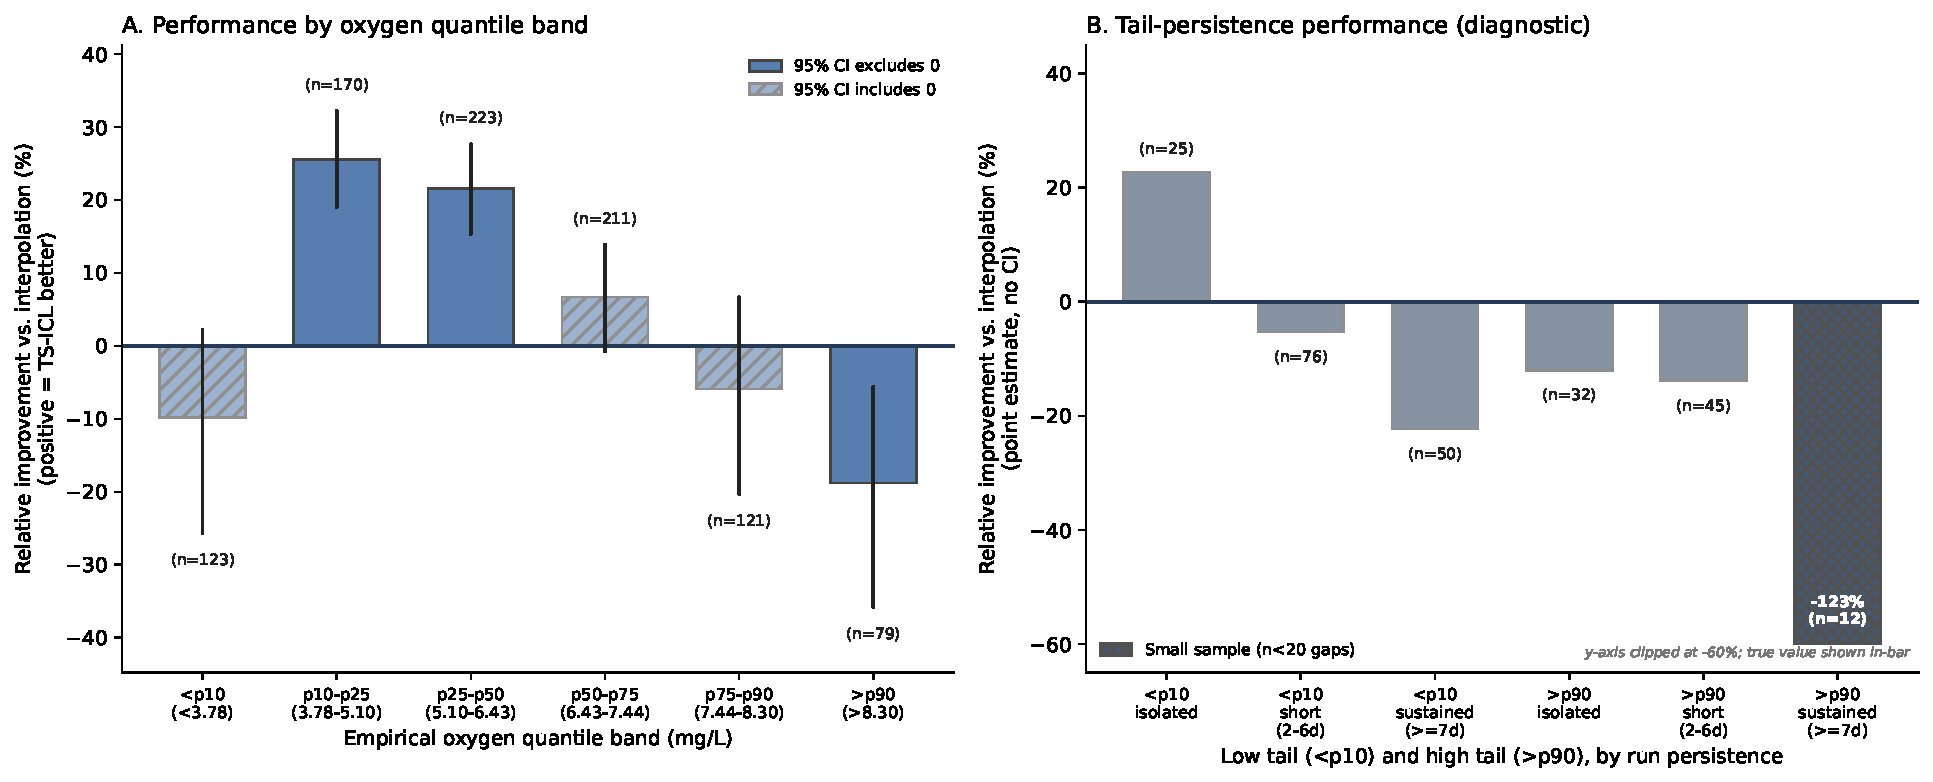
\includegraphics[width=\textwidth]{figures/fig_oxygen_tail_diagnostics_v6.pdf}
  \caption{Dissolved-oxygen distribution-tail diagnostics.
  (A) Relative improvement of the strongest TS-ICL arm over interpolation across empirical
  oxygen quantile bands. (B) Tail-persistence diagnostic for low-oxygen and high-oxygen tail runs. Quantile bands are empirical validation strata, not ecological
  thresholds.}
  \label{fig:oxygen_tail_diagnostics}
\end{figure}
